\documentclass[12pt]{article}
	
\usepackage[margin=1in, left=0.6in, right=0.6in]{geometry}	
\usepackage{fancyhdr}
\usepackage{relsize}
\usepackage[table]{xcolor}
\usepackage{graphicx} \graphicspath{ {./images/} }
\usepackage{amsmath,amsthm,amssymb}	%one of them is \text

\pagestyle{fancy}
\fancyhead[LO,L]{CSCB58 Lab 5}
\fancyhead[CO,C]{Stephen Guo}
\fancyhead[RO,R]{1006313231}
\fancyfoot[LO,L]{}
\fancyfoot[CO,C]{\thepage}
\fancyfoot[RO,R]{}

\setlength\extrarowheight{3pt}

%CSCB58_Lab5_StateDiagram.png
%\relscale{1}

\begin{document}
{\LARGE \noindent \underline{\textbf{Lab 5}}}
\begin{center}
    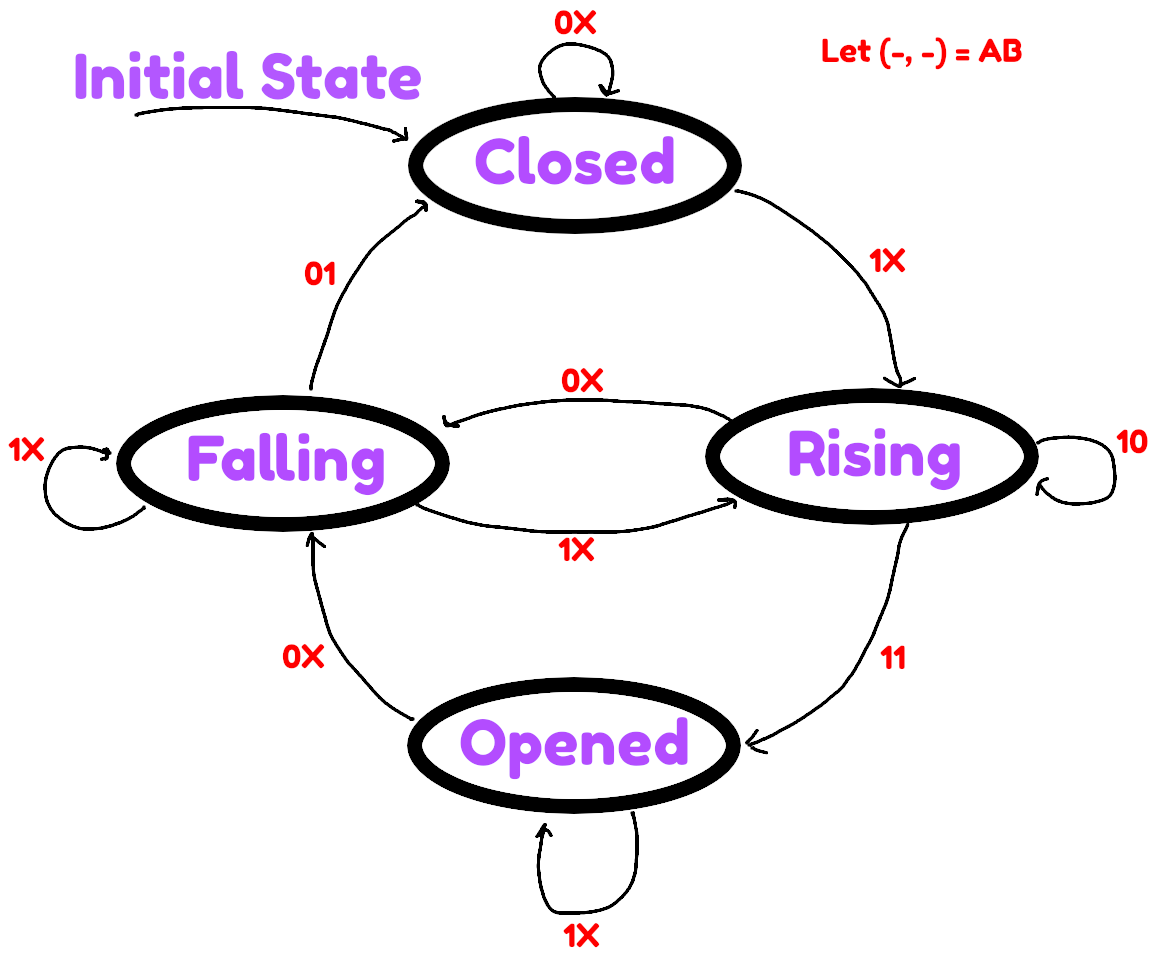
\includegraphics[width=14cm]{CSCB58_Lab5_StateDiagram.png} %width=\textwidth
    \\[1.5cm]
% \begin{center}
%     {\large State Transition Diagram}\\\ \\
%     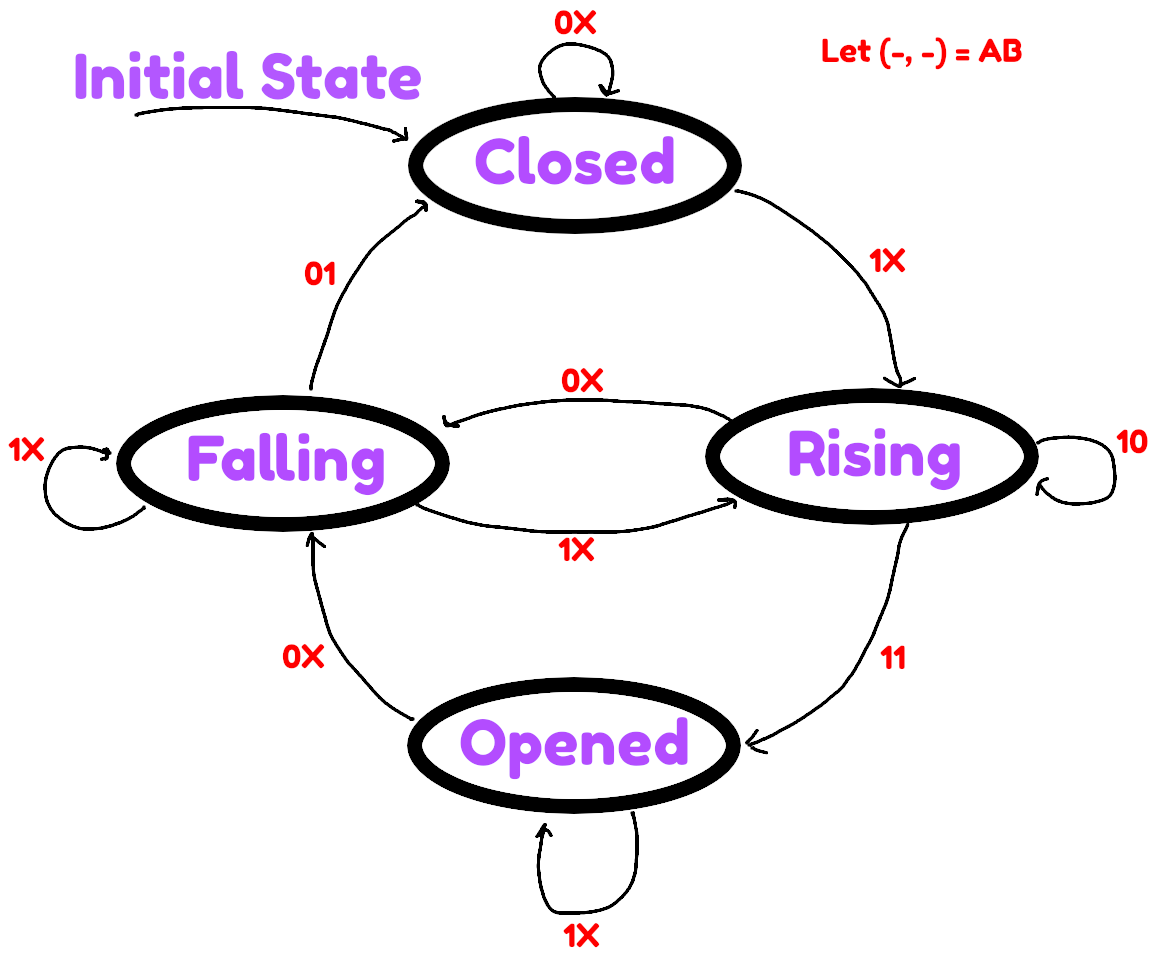
\includegraphics[width=14cm]{CSCB58_Lab5_StateDiagram.png} %width=\textwidth
%     \\\ \\
%     \begin{tabular}{|c|c|c|}
%         \hline 
%         \multicolumn{3}{|c|}{\cellcolor{gray!25}State Table}\\
%         \hline
%         \hline
%         \cellcolor{gray!25}Previous State & \cellcolor{gray!25}Input & \cellcolor{gray!25}Next State \\
%         \hline \hline 
%         Closed&0&0   \\ \hline
%         Closed&0&1  \\ \hline
%         Closed&0&1  \\ \hline
%         Rising&1&0   \\ \hline
%         Rising&1&1   \\ \hline
%         Rising&1&1   \\ \hline
%         Opened&X&X   \\ \hline
%         Opened&X&X   \\ \hline
%         Opened&X&X   \\ \hline
%         Falling&X&X   \\ \hline
%         Falling&X&X   \\ \hline
%         Falling&X&X   \\ \hline
%     \end{tabular}
% \end{center}

% \newpage
% \begin{center}
%     \begin{tabular}{|c|c|c|}
%         \hline 
%         \multicolumn{3}{|c|}{\cellcolor{gray!25}State Table}\\
%         \hline
%         \hline
%         \cellcolor{gray!25}Previous State & \cellcolor{gray!25}Input $(R, L)$& \cellcolor{gray!25}Next State \\
%         \hline \hline 
%         Closed&(0,\ 0)&Closed   \\ \hline
%         Closed&(1,\ 0)&Rising\\ \hline
%         Rising&(1,\ 0)&Rising\\ \hline
%         Rising&(0,\ 1)&Falling\\ \hline
%         Rising&(0,\ 0)&Opened\\ \hline
%         Opened&(0,\ 0)&Opened\\ \hline
%         Opened&(0,\ 1)&Falling\\ \hline
%         Falling&(0,\ 1)&Falling\\ \hline
%         Falling&(1,\ 0)&Rising\\ \hline
%         Falling&(0,\ 0)&Closed\\ \hline
%     \end{tabular}
%     \\[1cm] \newpage
%     \begin{tabular}{|c|c|c|}
%         \hline 
%         \multicolumn{3}{|c|}{\cellcolor{gray!25}State Table}\\
%         \hline
%         \hline
%         \cellcolor{gray!25}Previous State & \cellcolor{gray!25}Input $(R, L)$& \cellcolor{gray!25}Next State \\
%         \hline \hline 
%         Closed&(0,\ X)&Closed   \\ \hline
%         Closed&(1,\ X)&Rising\\ \hline
%         Rising&(1,\ X)&Rising\\ \hline
%         Rising&(0,\ 1)&Falling\\ \hline
%         Rising&(0,\ 0)&Opened\\ \hline
%         Opened&(X,\ 0)&Opened\\ \hline
%         Opened&(X,\ 1)&Falling\\ \hline
%         Falling&(X,\ 1)&Falling\\ \hline
%         Falling&(1,\ 0)&Rising\\ \hline
%         Falling&(0,\ 0)&Closed\\ \hline
%     \end{tabular}
%     \\[1cm]
%     {$$\begin{array}{r@{}>{\displaystyle}l}
% 		\text{Closed}&{} \rightarrow 00\\
%         \text{Rising}&{} \rightarrow 10\\
%         \text{Opened}&{} \rightarrow 11\\
%         \text{Falling}&{} \rightarrow 01\\
% 	\end{array}$$}\\[1cm]
%     Closed $\rightarrow 00$ \\
%     Rising $\rightarrow 10$ \\
%     Opened $\rightarrow 11$ \\
%     Falling $\rightarrow 01$ \\ \newpage

%     \begin{tabular}{|c|c||c|c||c|c|}
%         \hline 
%         \multicolumn{6}{|c|}{\cellcolor{gray!25}State Table}\\
%         \hline
%         \hline
%         \cellcolor{gray!25} F1& \cellcolor{gray!25}F0& \cellcolor{gray!25}IN1& \cellcolor{gray!25}IN0& \cellcolor{gray!25}newF1& \cellcolor{gray!25}newF0 \\
%         \hline \hline 
%         0&0&0&X&0&0\\ \hline
%         0&0&1&X&1&0\\ \hline
%         1&0&1&X&1&0\\ \hline
%         1&0&0&1&0&1\\ \hline
%         1&0&0&0&1&1\\ \hline
%         1&1&X&0&1&1\\ \hline
%         1&1&X&1&0&1\\ \hline
%         0&1&X&1&0&1\\ \hline
%         0&1&1&0&1&0\\ \hline
%         0&1&0&0&0&0\\ \hline
%     \end{tabular}\newpage \noindent
    \begin{tabular}{|c|c|c|}
        \hline 
        \multicolumn{3}{|c|}{\cellcolor{gray!25}State Table}\\
        \hline
        \hline
        \cellcolor{gray!25}Previous State & \cellcolor{gray!25}Input $(A, B)$& \cellcolor{gray!25}Next State \\
        \hline \hline 
        Closed&(0,\ X)&Closed   \\ \hline
        Closed&(1,\ X)&Rising\\ \hline
        Rising&(1,\ 0)&Rising\\ \hline
        Rising&(0,\ X)&Falling\\ \hline
        Rising&(1,\ 1)&Opened\\ \hline
        Opened&(1,\ X)&Opened\\ \hline
        Opened&(0,\ X)&Falling\\ \hline
        Falling&(0,\ 0)&Falling\\ \hline
        Falling&(1,\ X)&Rising\\ \hline
        Falling&(0,\ 1)&Closed\\ \hline
    \end{tabular}\newpage
    {$$\begin{array}{r@{}>{\displaystyle}l}
		\text{Closed}&{} \rightarrow 00\\
        \text{Rising}&{} \rightarrow 10\\
        \text{Opened}&{} \rightarrow 11\\
        \text{Falling}&{} \rightarrow 01\\
	\end{array}$$}\\[1.5cm]
    \begin{tabular}{|c|c||c|c||c|c|}
        \hline 
        \multicolumn{6}{|c|}{\cellcolor{gray!25}Truth Table}\\
        \hline
        \hline
        \cellcolor{gray!25} F1& \cellcolor{gray!25}F0& \cellcolor{gray!25}A& \cellcolor{gray!25}B& \cellcolor{gray!25}newF1& \cellcolor{gray!25}newF0 \\
        \hline \hline 
        0&0&0&X&0&0\\ \hline
        0&0&1&X&1&0\\ \hline
        1&0&1&0&1&0\\ \hline
        1&0&0&X&0&1\\ \hline
        1&0&1&1&1&1\\ \hline
        1&1&1&X&1&1\\ \hline
        1&1&0&X&0&1\\ \hline
        0&1&0&0&0&1\\ \hline
        0&1&1&X&1&0\\ \hline
        0&1&0&1&0&0\\ \hline
    \end{tabular}\\[2cm]
    \begin{tabular}{|c|c||c|c|}
        \hline 
        \multicolumn{4}{|c|}{\cellcolor{gray!25}Output Logic}\\
        \hline
        \hline
        \cellcolor{gray!25} F1& \cellcolor{gray!25}F0& \cellcolor{gray!25}R& \cellcolor{gray!25}L \\
        \hline \hline 
        0&0  &  0&0\\ \hline
        1&0  &  1&0\\ \hline
        1&1  &  0&0\\ \hline
        0&1  &  0&1\\ \hline

    \end{tabular} 

\end{center}
\end{document}